%     Železniční zabezpečovací technika
% notes:
%~~~~~~~~~
% notes:
%~~~~~~~~~
% \label{zzt:eq000}
% \label{zzt:fig001}
% \label{zzt:exam000}
% \label{zzt:tab000}
%---------------------------------------------------------------------------------------------------
% Setting path to image 
\graphicspath{{../src/ZZT/img/}}
%---------------------------------------------------------------------------------------------------
% file ZZT.tex
%--------------------------------------------------------------------------------------------------
\part{BZT}\label{part:BZT}
\parttoc

\ifthenelse{ \equal{\DebugMode}{true} }{
% Debug mode ON
  % !TeX spellcheck = cs_CZ
%{\tikzset{external/prefix={tikz/PZT/}}
% \tikzset{external/figure name/.add={ch02_}{}}
%---------------------------------------------------------------------------------------------------
% file ra3ch001.tex
%---------------------------------------------------------------------------------------------------
%======================== Kapitola: Železniční zabezpečovací technika ============================
%\begin{Czech}
\chapter{Obsah zabezpečovací techniky}\label{bzt:chapI}
\minitoc
  Důležitým odvětvím v železniční dopravě je odvětví zabezpečovací techniky. Potřeba zabezpečení 
  železničního provozu vznikala již v prvních začátcích železniční dopravy, ale postupný rozvoj 
  železniční dopravy si vynutil stále větší požadavky na konstrukci nových druhů zařízení a na 
  odbornost pracovníků pro jejich obsluhu.
  
  Tyto příručka je určena jako studijní materiál nezbytný pro implementaci moderních 
  metod návrhu zabezpečovacích systémů v železniční dopravě. 
   
\section{Náplň zabezpečovací techniky}
  Klasická železniční zabezpečovací zařízení jsou definována jako zařízení, která prvořadě 
  kontrolují, zda zamýšlené disposice dopravních zaměstnanců jsou bezpečné a zda jím nařízené 
  výkony se provádějí tak, aby nebyla ohrožena bezpečnost železniční dopravy. Pro přiblížení 
  uvažujme část stanice podle obr. \ref{zzt:fig001} a na této situaci s určitými zjednodušeními 
  tento obsah naznačme.

  \begin{figure}[ht!] %\ref{zzt:fig001}
    \centering
    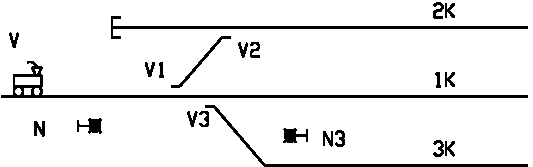
\includegraphics[width=0.8\linewidth]{zzt_fig001.pdf}
    \caption{Stanice
             (\cite[s.~5]{Chudacek2005})}
    \label{zzt:fig001}
  \end{figure}
 
  Před stanicí je umístěno návěstidlo \(N\), které v základní poloze ukazuje návěst \uv{stůj}. Dokud
  návěstidlo ukazuje tuto návěst, nesmí vlak \(V\) do stanice vjet. Má-li vlak vjet bezpečně např. 
  na kolej \(1K\), je třeba splnit určité podmínky. Výměny - pohyblivé části výhybek - \(V1\) a 
  \(V3\) musí být v poloze umožňující řádnou jízdu na kolej \(1K\), tj. jeden jazyk musí
  vždy přiléhat k příslušné opornici, druhý musí být od své opornice náležitě vzdálen. Na koleji 
  \(1K\) (včetně výhybek \(V1\) a \(V3\)) nesmí být žádná vozidla a ani nesmí být povolen příjezd
  jiných vozidel na tuto kolej z opačného směru. Zamýšlenou cestu nesmí ohrožovat z boku pohyby 
  jiných vlaků nebo posunujících dílů, proto výměna \(V2\) musí kolizní jízdu svou polohou 
  znemožňovat a návěstidlo \(N3\) musí kolizní jízdu zakazovat (ochrana odvratnou polohou výměny se 
  nazývá \emph{přímou boční ochranou}, ochrana návěstidlem se zakazující návěstí je \emph{nepřímou 
  boční ochranou}). Když tedy byly všechny prvky zvolené cesty správně nastaveny, přezkoušeny a 
  shledány bez závady, může být návěstidlo \(N\) přestaveno do polohy dovolující jízdu. Po celou 
  dobu, kdy návěstidlo dovoluje jízdu, bude dohlíženo, že všechny k tomu rozhodující podmínky jsou 
  nadále splněny. Vlak \(V\) vjede do stanice a ihned po jeho vjezdu se návěstidlo \(N\) přestaví 
  opět do základní polohy (návěst "stůj"), aby týž povel návěstidla nemohl být využit více vlaky a 
  aby shora uvedený postup bylo třeba pro každý vlak znovu opakovat.

  \begin{figure}[ht!] %\ref{zzt:fig002}
    \centering
    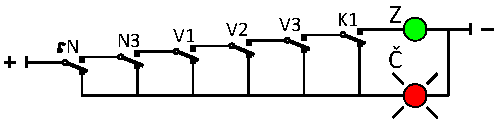
\includegraphics[width=0.8\linewidth]{zzt_fig002.pdf}
    \caption{Vybavení koleje technickým zařízením, které dohlíží na aby vlak vjel do stanice 
             bezpečně
             (\cite[s.~5]{Chudacek2005})}
    \label{zzt:fig002}
  \end{figure}
  
  Úkony, potřebné k tomu, aby vlak vjel do stanice bezpečně, může vykonat určený zaměstnanec. Ten
  se například pochůzkou přesvědčí, že kolej \(1K\) je volná, že výměny jsou řádně postaveny atd. a 
  po ověření všech podmínek přestaví návěstidlo \(N\) do polohy povolující jízdu. Pokud se 
  zaměstnanec nezmýlí, nedojde k nehodě (povšimněme si, že negace této věty nemusí být pravdivá). 
  Bezpečnost jízdy vlaku bude tedy závislá na osobních vlastnostech člověka. Aby tomu tak nebylo, 
  vybavíme koleje technickým zařízením, které bude na jejich volnost dohlížet, výměny jinými
  technickými zařízeními, která budou kontrolovat jejich polohu atd. a jízdní návěst návěstidel
  učiníme nuceně závislou na informacích těchto technických zařízení. Primitivní schéma
  takového zařízení je na obr. \ref{zzt:fig002}. I když pak dopravní zaměstnanec dá návěstním 
  řadičem \(N\) pokyn k rozsvícení jízdní (tj. jízdu povolující) návěsti \(Z\), návěst se rozsvítí 
  jen v případě, že kontakt \(N3\) informuje svým sepnutím, že návěstidlo \(N3\) skutečně ukazuje 
  návěst "stůj", kontakty \(V1\), \(V2\) a \(V3\) informují, že výměny jsou ve správné poloze a 
  kontakt \(K1\) informuje, že první kolej je volná a není na ni postavena jiná cesta. Jízdní 
  návěst \(Z\) se tedy rozsvítí až po splnění všech předem stanovených podmínek pro bezpečný vjezd 
  vlaku. Není-li kterákoliv podmínka splněna, na návěstidle \(N\) zůstává svítit červené světlo Č. 
  
  Přesto takové zařízení \textbf{nelze} považovat za zabezpečovací zařízení. Prvním důvodem je, že 
  nebyly zřízeny \emph{vzájemné závislosti}. Jízdní návěst na návěstidle \(N\) se sice rozsvítí až 
  když jsou splněny všechny podmínky, ale výměny a návěstidla zůstala volná. Nic nebrání, aby se 
  např. poloha výměn změnila dříve, než vlak \(V\) ukončí svou jízdu. Zhasnutí jízdního znaku \(Z\) 
  na návěstidle \(N\) v důsledku ztráty kontroly při přestavení výměny už nemusí být nic platné, 
  protože vlak již mohl návěstidlo minout nebo již není schopen včas zastavit. Nepostačí ale ani 
  zřízení vzájemné závislosti tím, že by rozsvícená jízdní návěst \(Z\) uzavírala výměny a 
  návěstidla v žádoucí poloze (např. prostřednictvím sériově řazeného relé). Vzhledem k nebezpečí
  přerušení sekvence postupných kroků je důležité, aby uzavření výměn a návěstidel bylo provedeno 
  dříve, než se rozsvítí jízdní návěst. Postup stavění jízdní cesty, vyhovující požadavkům 
  zabezpečovací techniky, bude tedy v naznačeném příkladě následující:
  \begin{itemize}\addtolength{\itemsep}{-0.5\baselineskip}
    \item nejprve se přestaví výměny do žádané polohy,
    \item v druhém úkonu (nazývaném závěr jízdní cesty) se při uzavírání výměn a návěstidel 
          přezkouší jejich správná poloha a tedy, že první úkon byl řádně proveden. Pokud první 
          úkon nebyl proveden správně, musí být znemožněn úkon druhý,
    \item obdobně třetí úkon, tj. rozsvícení jízdní návěsti na návěstidle \(N\), je možný jen 
          tehdy, byl-li druhý úkon (a tedy i první úkon) řádně proveden. 
  \end{itemize}
  
  Tím jsme dosáhli požadované \emph{vzájemné závislosti}, jejíž popsaná úroveň je \textbf{prvním
  charakteristickým rysem} zabezpečovacího zařízení. Zařízení z obr. \ref{zzt:fig002} bude podmínce 
  vyhovovat například v případě, že návěstní přepínač \(N\) bude konstrukčně upraven tak, že ho 
  nebude možné přeložit bez provedení \textbf{závěru jízdní cesty}. Důsledkem zavedení závěru 
  jízdní cesty bude potřeba po vlaku jízdní cestu vybavit, tj. závěr zrušit, aby bylo možné s 
  jednotlivými prvky opět volně manipulovat. 

  Ani nyní však ještě nelze v uvedeném příkladě hovořit o zabezpečovacím zařízení. Zařízení musí
  být konstruováno tak, aby \emph{bezpečnost byla zachována i při jakékoliv možné poruše vlastního 
  zařízení}. Tento  požadavek platí jak pro jednotlivé části, tak pro celek a je \textbf{druhým 
  charakteristickým rysem} železniční zabezpečovací techniky. V uvedeném případě to znamená, že 
  zařízení pro kontrolu volnosti koleje nesmí ani při poruše hlásit obsazenou kolej jako volnou, 
  zařízení pro kontrolu polohy výměny nesmí ani při poruše hlásit nesprávně postavenou výměnu jako 
  výměnu správně postavenou, ke zrušení závěru jízdní cesty nesmí ani poruchou dojít dříve než vlak 
  dotčené prvky skutečně mine atd. Právě tak vlastní zapojení pro rozsvícení jízdní návěsti musí 
  být konstruováno tak, aby se jízdní návěst nemohla poruchou zapojení rozsvítit, pokud všechny 
  podmínky pro její svícení nebudou splněny. Jak patrno, vychází se ze základního železničního
  bezpečnostního předpokladu, že zastavení vlaku poskytuje nejvyšší bezpečnost. Tento předpoklad se 
  zásadně liší od principů aplikovaných v letecké dopravě, kosmonautice, nukleární technice, 
  navigaci, řízení procesů, robotice, dolování, systémech zabezpečení proti vloupání či odcizení 
  atd., kde je prozatím obvykle hlavním cílem dosažení maximální spolehlivosti a pohotovosti 
  systému.
  
  Důsledkem druhého charakteristického rysu zabezpečovací techniky, tj. převedení všech poruch
  bezpečnějším směrem je, že téměř každá porucha zabezpečovacího zařízení znamená omezení dopravy. 
  To samozřejmě může vést k narušení plynulosti a vzniku provozních nepravidelností, což jsou jevy, 
  které samy o sobě nebezpečí v dopravě výrazně zvětšují. Ve vážnějších případech je nutné 
  zabezpečovací zařízení do skončení jeho opravy zcela vypnout, aby byl možný alespoň omezený pohyb 
  vlaků. Pak se ovšem provoz, jehož pravidelnost je navíc narušena, děje bez jakékoliv podpory 
  zabezpečovacího zařízení, zatížen, byť i jen na omezenou dobu, možnými lidskými omyly. Odtud tedy 
  plyne třetí charakteristický rys zabezpečovací techniky, což je taková konstrukce zařízení, která 
  má co nejméně poruch, tedy vysokou spolehlivost nebo - obecněji - co nejvyšší pohotovost. 
 
  Úloha zabezpečovací techniky nekončí zajištěním odpovídajícího návěstního znaku na návěstidle.
  Také na lokomotivě je strojvedoucí, jemuž je svěřena péče o bezpečnost vlaku a který tuto 
  bezpečnost může ohrozit svým omylem. Působnost zabezpečovacích zařízení se tedy (prostřednictvím 
  vlakového zabezpečovacího zařízení) prodlužuje až na vozidlo, aby se zajistilo, že vlak také 
  skutečně bude návěsti respektovat. 

  Aplikují-li se všechny výše uvedené zvláštnosti správně při vývoji zabezpečovacího systému, je
  třeba se postarat také o to, aby nedošlo k jejich znehodnocení při projekci, výrobě, montáži a 
  údržbě konkrétních zařízení. Při těchto činnostech je také třeba počítat s lidskými vlastnostmi. 
  Zařízení, sloužící primárně pro eliminaci chyb dopravních zaměstnanců konstruují, vyrábějí, 
  montují a udržují opět lidé. Naštěstí tyto práce, na rozdíl od výkonu dopravní služby, probíhají 
  (nebo by rozhodně měly probíhat) v lepších podmínkách a bez časové tísně. Za příznivých podmínek 
  se nedokonalosti člověka tolik neuplatňují a práci každého pracovníka lze kontrolovat jinými s 
  případnou pomocí dalších technických zařízení. Přesto však z toho pro projekci, výrobu, montáž a 
  údržbu zabezpečovacích zařízení vyplývají jisté zvláštnosti. 
  
  Vedle úloh z oblasti bezpečnosti plní moderní zabezpečovací technika i úkoly další. Především jde
  o hlubší zásahy do vlastního provozu prostředky automatizace. Ta pak, při správném provedení, 
  vede k zlepšenému využití technických prostředků železnic (např. zvýšení propustné výkonnosti 
  tratí), k zhospodárnění provozu, k úspoře jiných, podstatně vyšších investičních nákladů (např. 
  budování další koleje). Protože však zabezpečovací zařízení je zařízením v zásadě restriktivním, 
  nelze u něj bezhlavě prosazovat zvyšování výkonnosti vždy a ve všech směrech. Později také 
  uvidíme, že zabezpečovací technika se podílí na zvyšování bezpečnosti i v jiných oblastech: 
  kolejové obvody alespoň částečně dohlíží na stav jízdní dráhy (celistvost kolejnic), přestavná 
  zařízení výměn dohlíží na stav výhybek, vlakové zabezpečovače mohou do určité míry dohlížet na 
  stav brzdové soustavy vlaku (sledováním skutečně dosaženého odrychlení při brzdění), přejezdová 
  zabezpečovací zařízení se podílejí na eliminaci cizích vlivů na dopravu atd.
  
  Souhrnně lze konstatovat, že prvořadým účelem zabezpečovacích zařízení na železnici je
  předcházet kolizím a vykolejení vlaků z důvodu chybného řízení dopravy. K tomu účelu je u 
  zařízení třeba sledovat následující oblasti:
  \begin{itemize}\addtolength{\itemsep}{-0.5\baselineskip}
    \item funkční bezpečnost (korektnost systému), tj. řádné plnění všech požadovaných funkcí v 
          bezporuchovém stavu a při očekávaných vlivech pracovního prostředí,
    \item technickou bezpečnost (bezpečnou konstrukci), tj. splnění požadavku, aby nedošlo k 
          přímému ohrožení bezpečnosti dopravy ani při poruchách samotného zabezpečovacího zařízení,
    \item bezpečnou aplikaci, tj. vytvoření takových logických funkcí a vzájemných závislostí, aby 
          pro konkrétní situaci navržené zařízení ve všech provozních stavech mohlo řádně plnit 
          svou funkci (na jeho výstupech budou jízdu povolující informace pouze v takovém rozsahu, 
          který odpovídá stavu informací vstupních) a zajištění, aby tyto vlastnosti zařízení mělo 
          i po výrobě a montáži,
    \item bezpečný provoz a údržbu, tj. zajištění, že předchozí úrovně zůstanou v zařízení 
          zachovány po celou dobu životnosti,
    \item vysokou spolehlivost, tj. omezení případů, kdy nepřímo, vyřazením zabezpečovacího 
          zařízení a přechodem na manuální řízení, by mohlo dojít k ohrožení bezpečnosti dopravy.
  \end{itemize}
  Žádnou ze zmíněných oblastí nelze preferovat, protože žádná nemůže nahradit druhou a             
  nedostatky v kterékoliv z nich znehodnocují výsledky ostatních.
  
  Přímým obsahem železniční zabezpečovací techniky není zajištění zdraví a bezpečnosti
  zaměstnanců (i když provozovaná zařízení samozřejmě musí splňovat i požadavky např. ve směru 
  ochrany před nebezpečným dotykovým napětím, ergonomicky správně navrženého obsluhovací pracoviště 
  atd.), zabránit nehodám ze zlého úmyslu, násilnou obsluhou, úmyslným poškozením nebo zneužitím 
  zařízení. V poslední době se však jeví jako nezbytné dokonaleji zajišťovat zabezpečovací zařízení 
  proti vandalům a lapkům všeho druhu a neoprávněným zásahům do zařízení v případě, že používají 
  jiných než speciálně drážních zařízení (viz dále např. ochrana dat v otevřených sítích).  

\section{Třídění}
  K železničním zabezpečovacím zařízením se obvykle řadí i zabezpečovací zařízení používaná na
  podzemních drahách (metro, doly), na pouličních drahách (tramvaje - zejména městské rychlodráhy) 
  a na vlečkách, protože využívají obdobných principů, často i obdobná nebo jen poněkud upravená 
  zařízení. Při třídění zařízení lze použít řadu třídících hledisek; téměř vždy se však vyskytnou 
  zařízení přechodová (smíšená) nebo podle užitého třídění obtížně definovatelná. Přesto je dále 
  několik třídění uvedeno, protože poskytují obrázek o pestrosti a mnohotvárnosti pojednávaného 
  zařízení. 
  
  Nejpřirozenějším a klasickým tříděním zabezpečovacích zařízení je třídění podle účelu zařízení.
  Podle tohoto hlediska lze zabezpečovací zařízení dělit na zařízení: 
  \begin{itemize}\addtolength{\itemsep}{-0.5\baselineskip}
    \item staniční,
    \item traťové,
    \item vlakové,
    \item přejezdové, 
    \item spádovištní. 
  \end{itemize}
  Účel je patrný již z názvu. Staniční zabezpečovací zařízení zajišťuje bezpečný pohyb vlaků ve 
  stanici, traťové zařízení zabezpečuje jízdu vlaku na trati mezi stanicemi, vlakové zařízení 
  zabraňuje vlaku pohybovat se nad rámec, který povoluje zařízení staniční a traťové (s případným 
  zahrnutím i dalších omezení), přejezdové zařízení přispívá k zajištění bezpečnosti na úrovňovém 
  křížení silnice a železnice informováním uživatelů silnice, že se k přejezdu blíží vlak s 
  předností v jízdě. Nad všemi těmito zařízeními pak může být budováno zařízení pro dálkové 
  ovládání většího úseku tratě z jednoho místa. 
  
  Podle místa ovládání zařízení mluvíme o zařízení s obsluhou :
    \begin{itemize}\addtolength{\itemsep}{-0.5\baselineskip}
    \item místní,
    \item ústřední (centralizovanou v oblasti jedné stanice),
    \item dálkovou (mimo vlastní stanici).
  \end{itemize}

  Další třídění je odvozeno od způsobu ovládání periferií (výměn, návěstidel atd.) a tak vlastně
  zahrnuje celou historii železniční zabezpečovací techniky. Rozeznáváme zařízení:
  \begin{itemize}\addtolength{\itemsep}{-0.5\baselineskip}
    \item mechanická (využívající výhradně lidské síly),
    \item elektrická,
    \item pneumatická,
    \item hydraulická. 
  \end{itemize}

  Obdobně, v následujícím třídění je rozhodující způsob, jímž se v zařízení potřebné závislosti
  realizují. Zde rozeznáváme zařízení se závislostmi:
  \begin{itemize}\addtolength{\itemsep}{-0.5\baselineskip}
    \item mechanickými,
    \item mechanickými i elektrickými (tzv. elektromechanická a elektrodynamická zařízení),
    \item elektrickými, která lze dále dělit podle rozhodujících stavebních prvků, jimiž jsou 
         závislosti realizovány, na zařízení:
       \begin{itemize}
       \item reléová,
       \item hybridní (rozhodující část bezpečné logiky je realizována reléově, zbytek 
             elektronicky),
       \item elektronická (mikroprocesorová). 
       \end{itemize}
  \end{itemize}

  U traťových zabezpečovacích zařízení je kladen důraz na rozsah spolupůsobení vlaku. Zařízení se
  pak dělí na:
  \begin{itemize}\addtolength{\itemsep}{-0.5\baselineskip}
    \item poloautomatická (poloautobloky),
    \item automatická (autobloky).
  \end{itemize}
  Podle rozmístění traťových zařízení podél trati lze automatická zařízení dále dělit na:
  \begin{itemize}\addtolength{\itemsep}{-0.5\baselineskip}
    \item decentralizovaná (funkční bloky jsou umístěny v každém návěstním bodě),
    \item částečně centralizovaná (funkční bloky jsou umístěny pouze ve vybraných bodech na trati),
    \item centralizovaná (zařízení je koncentrováno do stanic).
  \end{itemize}
  Vlaková zabezpečovací zařízení se dělí podle způsobu přenosu informací mezi tratí a hnacím
  vozidlem na zařízení:
  \begin{itemize}\addtolength{\itemsep}{-0.5\baselineskip}
    \item bodová,
    \item semiliniová,
    \item liniová. 
  \end{itemize}

  Podle způsobu kontroly souladu jízdy vlaku s přenášenými informacemi se vlaková zařízení dále 
  dělí na zařízení s kontrolou:
  \begin{itemize}\addtolength{\itemsep}{-0.5\baselineskip}
    \item bdělosti strojvedoucího,
    \item rychlosti vlaku.
  \end{itemize}
  
  Zařízení přejezdová se dělí podle způsobu výstrahy na přejezdová zařízení:
  \begin{itemize}\addtolength{\itemsep}{-0.5\baselineskip}
    \item mechanická,
    \item světelná bez závor,
    \item světelná se závorami.
  \end{itemize}
  
  U moderních systémů dělení zabezpečovacích zařízení na zařízení staniční, traťová, vlaková a
  přejezdová ztrácí smysl, protože systémy jsou komplexní, se společným jádrem řídícím jednotlivé 
  periférie a tyto celky pak tvoří nanejvýš podsystémy. Na obr. 3-1 je základní blokové schéma 
  takového systému. 
  \begin{figure}[ht!] %\ref{zzt:fig003}
    \centering
    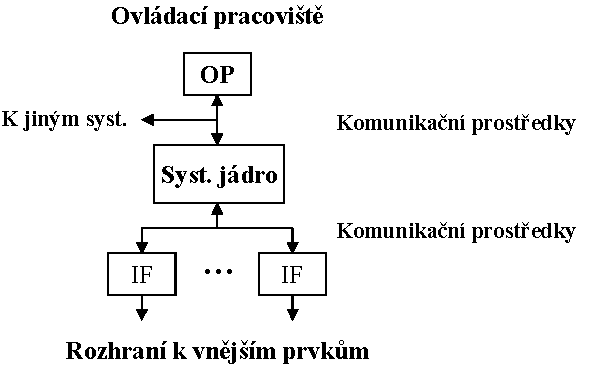
\includegraphics[width=0.8\linewidth]{zzt_fig003.pdf}
    \caption{Stanice
             (\cite[s.~11]{Chudacek2005})}
    \label{zzt:fig003}
  \end{figure}


  \section{Klasifikace poruch}
    \textbf{Chyba} je rozdíl mezi správnou a skutečnou hodnotou nějaké veličiny. V zařízení se 
    chyby mohou obecně objevit jako \emph{důsledek (projev) poruchy některé jeho součásti, 
    působením nějakého cizího vlivu} nebo \emph{selháním lidského činitele}. Za poruchy hardware se 
    považují všechna vybočení z předpokládaných vlastností stavebního prvku (součástky, dílu) 
    zařízení. Předpokládanými vlastnostmi prvků přitom jsou vlastnosti odpovídající příslušným 
    technickým podmínkám popisujícím jeho vlastnosti. Jako omyl lze označit každou lidskou činnost, 
    která může vést k nezamýšlenému chování zařízení. V širším slova smyslu se jako 
    \textbf{porucha} označují souhrnně všechny příčiny vedoucí k chybě, tj. poruch součásti, 
    cizí vliv i omyl.

%~~~~~~~~~~~~~~~~~~~~~~~~~~~~~~~~~~~~~~~~~~~~~~~~~~~~~~~~~~~~~~~~~~~~~~~~~~~~~~~~~~~~~~~~~~~~~~~~~~
\printbibliography[title={Seznam literatury}, heading=subbibliography]
\addcontentsline{toc}{section}{Seznam literatury}

\chapter{Bezpečnost a spolehlivost zabezpečovacích systémů}
 \section{Spolehlivost}
 \section{Bezpečnost}
    V různých publikacích je možné najít různé definice bezpečnosti. Například norma 
    EN~61508\footnote{Funkční bezpečnost elektrických/elektronických/programovatelných 
    elektronických systémů souvisejících s bezpečností (Functional safety of electrical/ 
    electronic/programmable electronic systems), obecná norma funkční bezpečnosti, která se opírá o 
    dvě základní koncepce - životní cyklus bezpečnosti a úroveň integrity bezpečnosti 
    (\texttt{SIL})} 
    definuje bezpečnost jako nepřítomnost netolerovaného rizika. Z této definice je zřejmé, že 
    bezpečnost je úzce spjatá s rizikem, a je nutné bezpečnost třeba chápat relativně. Když se 
    řekne, že řídicí systém je bezpečný, neznamená to jeho absolutní bezpečnost (ta je prakticky 
    nedosažitelná vzhledem na existenci objektivních faktorů, jako je například úroveň poznání, 
    technologická úroveň a limitované finanční prostředky), ale taková úroveň bezpečnosti, 
    která zodpovídá definovaným bezpečnostním požadavkům na tento řídicí systém. 

    Relativnost v pojímání bezpečnosti znamená posun od kvalitativního ke kvantitativnímu chápaní bezpečnosti.

    Kvalitativně je bezpečnost chápána jako schopnost řídicího systému zajistit omezení důsledků 
    poruch řídicích systému v daných podmínkách a v daném časovém intervalu. Matematicky je možné 
    kvalitativní bezpečnost řídicího systému vyjádřit jako 
    \begin{equation}
      E_H = 0,
    \end{equation}
    kde \(E_H\) je množina nebezpečných stavů, které jsou důsledkem výskytu pravděpodobných poruch 
    řídicího systému. Pravděpodobná porucha je taková porucha z množiny všech poruch, jejichž 
    výskyt během provozu řídicího systému je nutné předpokládat (vzhledem na požadovanou úroveň 
    bezpečnosti řídicího systému).
	
    Kvantitativně je bezpečnost řídicího systému chápána jako pravděpodobnost nepřítomnosti
    jakéhokoliv nebezpečného stavu v řídicím systému v daných podmínkách a v daném časovém
    intervalu. Je zřejmé, že i když pravděpodobnost nebezpečného stavu řídicího je malá, neznamená
    to, že se nebezpečný stav nemůže vyskytnou v nejbližším časovém intervalu, Matematicky je možné
    kvantitativní bezpečnost vyjádřit tak, že
    \begin{equation}
      P_{HT}(t)\geq P_{HT}(t)>0,
    \end{equation}
    kde \(P_{HT}(t)\) je pravděpodobnost tolerovaného nebezpeční řídicího systému a \(P_{HR}(t)\)
    je reálná pravděpodobnost nebezpeč\-ného stavu řídicího systému.
	 
    Na kvantitativním hodnocení bezpečnosti řídicího systému je v podstatě možné uplatnit stejné 
    teoretické postupy, jako při hodnocení spolehlivosti technických systémů. Zásadní rozdíl je v 
    tom, že při hodnocení spolehlivosti standardních řídicích systémů se obvykle rozlišují dva 
    stavy - bezporuchový stav a poruchový stav, a k těmto dvěma stavům se vztahují také 
    kvantitativní ukazatele spolehlivosti. Při hodnocení bezpečnosti řídicích systémů musíme 
    uvažovat s dvěma druhy poruchových stavů - bezpečným a nebezpečným poruchovým stavem. 
    Bezpečnost řídicího systému se potom vyjadřuje pomocí ukazatelů bezpečnosti (například 
    pravděpodobnost výskytu nebezpečné poruchy, intenzita nebezpečných poruch, ...).

    Při kvantitativním hodnocení důsledků poruch na bezpečnost řídicího systému se obvykle k 
    hodnoceným řídicím systémům přistupuje jako k neobnovovaným objektům, protože z pohledu 
    bezpečnosti jsou důležité dva stavy (bezpečný, nebezpečný) a analýza končí výskytem nebezpečné 
    poruchy (může jít o jednu poruchu, nebo o kombinaci více poruch, které nejsou individuálně 
    nebezpečné). To znamená, že od uvedení řídicího systému do provozu, až po výskyt nebezpečné 
    poruchy, se může řídicí systém střídavě nacházet ve funkčním, nebo nefunkčním stavu (nefunkční 
    ještě neznamená nebezpečný). Z tohoto důvodu ukazatele bezpečnosti jsou podobné ukazatelům 
    bezporuchovosti neobnovovaných objektů. 
  
    \subsection{Základní legislativa}
      \begin{itemize}
        \item \textbf{EN 61508} - \emph{základní všeobecná norma pro SRCS}; pojednává o funkční
              bezpečnosti elektrických/elektronických/programovatelných elektronických systémů
              souvisejících s bezpečností (Functional safety of electrical/electronic/programmable
              electronic systems), obecná norma funkční bezpečnosti, která se opírá o dvě základní
              koncepce - životní cyklus bezpečnosti a úroveň integrity bezpečnosti (\texttt{SIL})
              \begin{itemize}
                \item EN 61508-1: Všeobecné požadavky
                \item EN 61508-2: Požadavky na elektrické / elektronické / programovatelné
                                  elektronické systémy související s bezpečností
                \item EN 61508-3: Požadavky na SW
                \item EN 61508-4: Definice a zkratky
                \item EN 61508-5: Příklady metod určování úrovně integrity bezpečnosti
                \item EN 61508-6: Metodické pokyny na používání EN 61508-2, STN EN 61508-3
                \item EN 61508-7: Přehled technik a opatření
              \end{itemize}
        \item \textbf{EN 50126}: Railway applications – The specification and demonstration of
              reliability, availability, maintainability and safety (RAMS)
              \begin{itemize}
                \item Part 1: Basic requirements and generic process. 1999
                \item Part 2: Guide to the application of EN 50126-1 for safety. 2007
                \item Part 3: Guide to the application of EN 50126-1 for rolling stock RAMS. 2008  
              \end{itemize}
              Zabývá se specifikací parametrů RAMS (spolehlivost, pohotovost, udržovatelnost,
              a bezpečnost) obecně pro všechny železniční systémy, reaguje na skutečnost, že
              naléhavost požadavků na bezpečnost funkce jednotlivých železničních systémů je různá
              a lze je tedy splňovat s různou pravděpodobností jejich selhání. Také zavádí pojem
              \emph{integrita bezpečnosti (safety integrity - celistvost, úplnost, neporušenost
              bezpečnosti)}, který definuje jako pravděpodobnost, s níž systém uspokojivě splní
              požadované bezpečnostní funkce, za všech stanovených podmínek a ve stanoveném časovém
              období. Jde o to, do jaké míry může být pro bezpečnost relevantní funkce narušena
              např. poruchami vlastního zařízení, omyly obsluhy, vnějším rušením atd.
        \item \textbf{EN 50128}: Railway applications – Communication, signalling and processing
              systems – Software for railway control and protection systems. 2003          
        \item \textbf{EN 50129}: Railway applications – Communication, signalling and processing
              systems – Safety-related electronic systems for signalling. 2011
              Modifikovaně byl pojem integrita bezpečnosti přenesen i do této normy pro železniční
              zabezpečovací systémy. I klasická zabezpečovací technika bez velkého zdůrazňování
              respektovala, že nejsou na všechna zařízení kladeny stejně důrazné bezpečnostní
              požadavky (kategorie zařízení, vedlejší tratě/hlavní tratě, zařízení pro ČD/zařízení
              pro vlečky, staniční zařízení/spádoviště atd.). Uvidíme dále, že pojmu integrita
              bezpečnosti je pro zabezpečovací zařízení dominantně obsažena oblast, kterou běžně v
              této technice označujeme(a také normá EN 50129 ji tak označuje ve své základní části)
              termínem technická bezpečnost. Úvahy okolo integrity bezpečnosti zde sledujeme
              odděleně od úvah o technické bezpečnosti (přes jejich podobnost) pro jejich výhodnost
              zejména v úvodních fázích projektu nového systému (zařízení, výrobku, atd.)
        \item \textbf{EN 50159: Railway applications – Communication, signalling and processing
              systems - Safety-related communication in transmission systems. 2010}            
      \end{itemize}
    
      Vyjmenované normy se poněkud liší v definici termínu \emph{bezpečnost}:  
      \begin{itemize}
        \item Bezpečnost (Safety) – nepřítomnost nepřijatelných úrovní rizika poškození (EN50129)
        \item Bezpečnost (Safety) – nepřítomnost nepřijatelného rizika. (EN61508)
        \item Bezpečnost při poruše (Fail Safe) – vlastnost konstrukce objektu zabraňující,
              aby jeho poruchy způsobili nebezpečné poruchové stavy. (IEC 50 (191))
        \item Kvalitativní bezpečnost – schopnost systému zajistit omezení důsledku poruch
              systému v daných podmínkách a v daném časovém intervale.
        \item Kvantitativní bezpečnost – pravděpodobnost nepřítomnosti jakéhokoliv
              nebezpečného stavu v systéme v daných podmínkách a v daném časovém intervale.
      \end{itemize}

    \subsection{Ukazatel bezpečnosti}
      \fbox{Pravděpodobnost bezpečného provozu} je pravděpodobnost, že objekt může bezpečně plnit 
      požadovanou funkci v daných podmínkách v časovém intervalu \(t_1,\, t_2\).
      \begin{equation}
        R_S(t_1,\, t_2) = 1- F_H(t_1,\, t_2),
      \end{equation}
      kde \(F_H(t_1,\, t_2)\) je distribuční funkce, která naopak vyjadřuje pravděpodobnost, že
      objekt nemůže bezpečně plnit požadovanou funkci k daným podmínkám v časovém intervalu
      \(t_1,\, t_2\).
      \begin{equation}
        F_H(t_1,\, t_2) = \int_{t_1}^{t_2}f_H(t)\cdot\dd{t},
      \end{equation}
      kde \(f_H(t)\) je hustota pravděpodobnosti nebezpečné poruchy objektu. 

      \fbox{Intenzita nebezpečných poruch} \(\lambda_H(t)\) definujme jako limitu poměru podmíněné
      pravděpodobnosti, že časový okamžik vzniku nebezpečné poruchy objektu \(T\) padne do daného
      časového intervalu \(t,\, t+\Delta t\), přičemž délka časového intervalu \(\Delta
      t\rightarrow0\)
      \begin{equation}\label{DZT:eq_def_lambdaH}
        \lambda_H=\frac{f_H(t)}{R_S(t)}.
      \end{equation}

      Protože nebezpečné poruchy jsou méně časté, zkoušky na určení požadovaných ukazatelů
      bezpečnosti by bylo třeba provádět dlouhodobě, což je prakticky nemožné. 
    
  \section{Integrita bezpečnosti}
    Všeobecně je možné konstatovat, že SRCS realizuje řídící i ochranné funkce (obr.
    \ref{DZT:fig_DZT_SRCS_fce}). Jelikož selhání řídicí funkce může způsobit ohrožení bezpečnosti,
    je třeba i tyto funkce považovat za bezpečnostní.
    \begin{figure}[hb!]
      \centering
      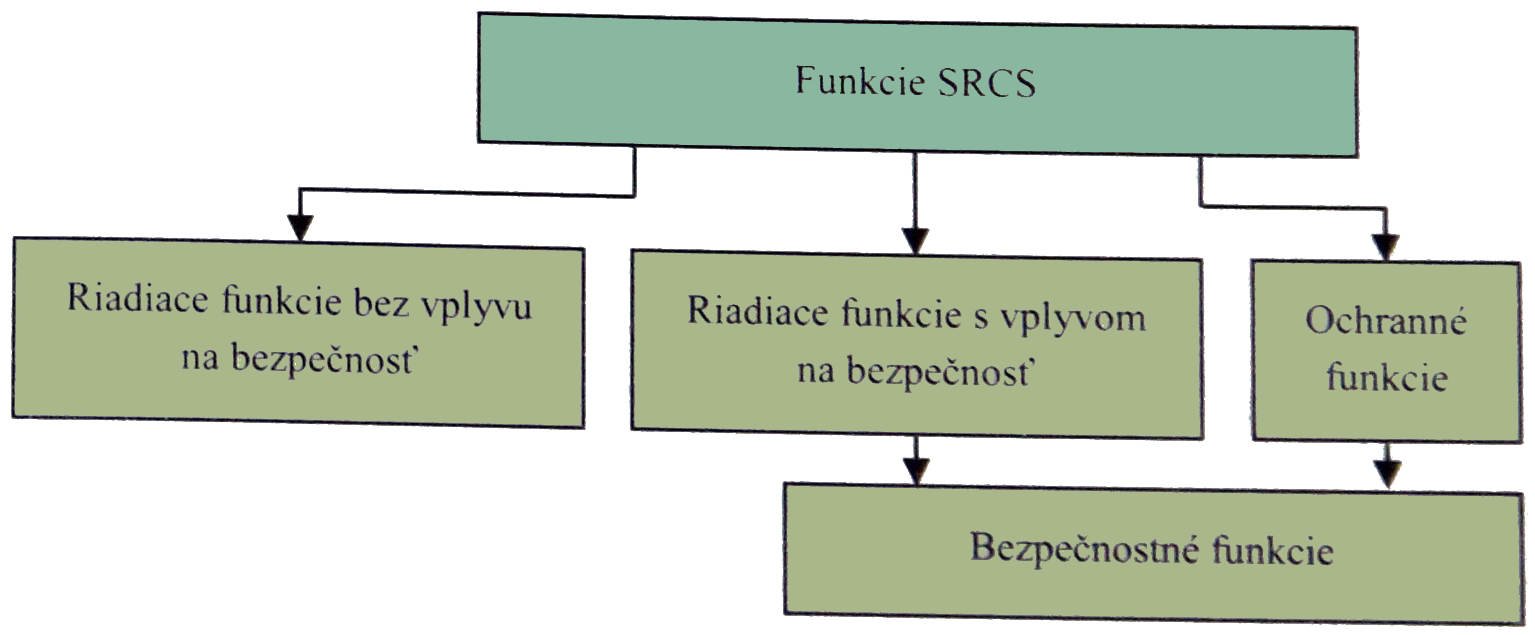
\includegraphics[width=1\linewidth]{DZT_SRCS_fce.jpg}
      \caption{Vztah mezi bezpečnostními funkcemi a moduly SRCS}
      \label{DZT:fig_DZT_SRCS_fce}
    \end{figure}    
    Bezpečnostní funkce jsou definované na základě analýzy rizik jako technická opatření na snížení
    rizika spojeného s konkrétními nebezpečí na tolerovatelnou úroveň. Účinnost bezpečnostní funkce
    se určuje pomocí úrovně integrity bezpečnosti \emph{(\texttt{SIL} - safety integrity level)}. 
    
    Norma \emph{EN 61508} definuje integritu bezpečnosti jako pravděpodobnost, že SRCS bude plnit 
    požadované bezpečné funkce za všech stanovených podmínek v rámci stanoveného operačního 
    prostředí a během stanoveného časového období. Všeobecně lze konstatovat, že čím je integrita
    bezpečnosti SRCS větší, tím je menší pravděpodobnost selhání bezpečností funkce realizovaných
    SRCS.  
    
    Integrita bezpečnosti se skládá ze dvou částí a to:
    \begin{itemize}
      \item \emph{integrity bezpečnosti proti systematickým poruchám}: jde o nekvantifikovatelnou
            část integrity bezpečnosti, která souvisí s nebezpečnými systematickými poruchami 
            hardware a software; integrity bezpečnosti proti systematickým poruchám se dosahuje
            především opatřeními na předcházení chybám a poruchám; vzhledem k tomu, že jde o 
            nekvantifikovatelnou část integrity bezpečnosti, je vhodnější chápat integritu 
            bezpečnosti jako vlastnost a né jako pravděpodobnost; hodnocení integrity bezpečnosti
            proti systematickým chybám a poruchám se realizuje kontrolou dodržování opatření
            předcházejících chybám a poruchám, mezi které patří také důsledné testování korektní
            realizace bezpečnostních funkcí; 
      \item \emph{integrity bezpečnosti proti náhodným poruchám}: jde o kvantifikovatelnou část
            integrity bezpečnosti, která se týká náhodných poruch hardware vyplývajících z konečné
            bezporuchovosti použitých součástek; hodnocení integrity bezpečnosti proti náhodným
            poruchám se realizuje prostřednictvím pravděpodobnostních výpočtů.
    \end{itemize}
    
    Aby se dosáhla požadovaná integrita bezpečnosti, musí být splněné požadavky na integritu proti 
    systematickým poruchám i náhodným poruchám. 
    
    \subsection{Úroveň integrity bezpečnosti}
      Úroveň integrity bezpečnosti (\emph{Safety Integrity Levels - \texttt{SIL}}) se dělí podle EN 
      50129
      do čtyř kategorií - úroveň 4 (\texttt{SIL} 4) je nejvyšší, úroveň 1 (\texttt{SIL} 1) je 
      nejnižší.  Pokud se
      objevuje úroveň \texttt{SIL} 0, značí to, že se jedná o systém na které nejsou kladeny žádné
      bezpečnostní požadavky (ve smyslu zabezpečovací techniky)
      
      Proto, aby SRCS mohl být zařazen do odpovídající úrovně bezpečnosti \texttt{SIL}, musí 
      vyhovovat
      těmto faktorům:
      \begin{itemize}
        \item naplnění podmínek řízení kvality, 
        \item naplnění podmínek řízené bezpečnosti,
        \item splnění požadavků na technickou bezpečnost, 
        \item dosažení kvantitativního cíle
      \end{itemize}
      
      Jak patrno, splnění kvantitativního ukazatele samo o sobě neznamená, že bylo dosaženo
      odpovídající úrovně bezpečnosti. To platí ovšem i naopak - splnění tří předchozích podmínek
      (řízení kvality, řízení bezpečnosti a technické bezpečnosti) nezaručuje, že bylo dosaženo
      kvantitativních cílů a nelze tedy tvrdit, že zařízení lze zařadit do odpovídající skupiny
      \texttt{SIL} (\ref{DZT:fig_EN50129_SIL_techniques}).
      
      \begin{figure}[ht!]% Relationship between \texttt{SIL}s and techniques
        \centering
        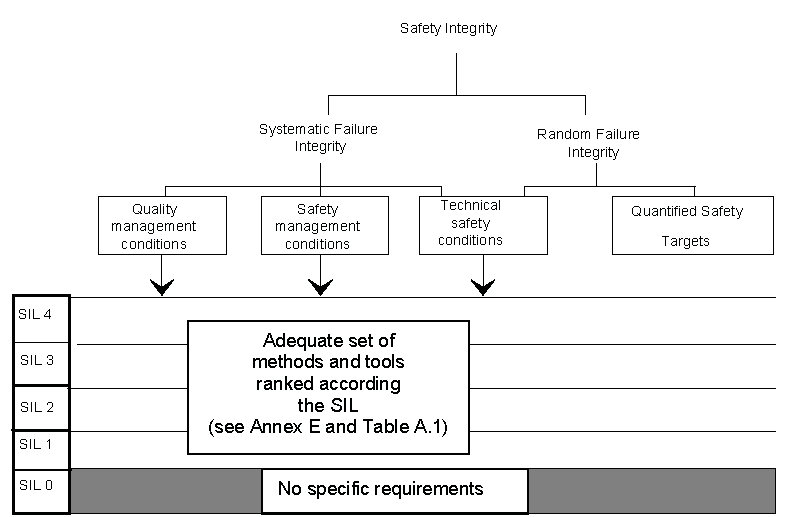
\includegraphics[width=0.95\linewidth]{EN50129_SIL_techniques.pdf}
        \caption{Vztah mezi \texttt{SIL} úrovní a technikami jejich dosažení}
        \label{DZT:fig_EN50129_SIL_techniques}
      \end{figure}
      
      Žádná z norem \texttt{CENELEC} nepředepisuje, které zařízení musí být jaké úrovně. Toto 
      určení je 
      ponecháno na provozovateli, resp. regulátorovi, vyplyne také z provedených analýz rizik 
      a hazardů.
      
      Následující tabulka shrnuje definované úrovně integrity bezpečnosti a zároveň dává do
      souvislosti s tolerovatelnými četnostmi hazardů. \texttt{SIL} jsou tedy prostředkem přiřazení
      kvalitativních přístupů (pro vyloučení systematických poruch) ke kvantitativnímu přístupu
      (pro řízení náhodných poruch), neboť systematické poruchy nelze kvantifikovat.
      \begin{table}[h]
        \centering
        \begin{tabular}{|c|c|}
          \hline
           Úroveň integrity &  Tolerovatelná četnost hazardu            \\
             bezpečnosti \texttt{SIL} &  THR [za hodinu a funkci]       \\ \hline\hline 
              4        & \(10^{-9}\leq THR < 10^{-8}\)                  \\ \hline
              3        & \(10^{-8}\leq THR < 10^{-7}\)                  \\ \hline
              2        & \(10^{-7}\leq THR < 10^{-6}\)                  \\ \hline
              1        & \(10^{-6}\leq THR < 10^{-5}\)                  \\ \hline
        \end{tabular}
        \caption{\texttt{SIL} tabulka: Funkce, jejichž kvantitativní požadavky by převyšovaly 
                 hranici \(10^{-9}\), která se zdánlivě nelogicky objevuje u \texttt{SIL4}, vyžaduje
                 podle normy \texttt{EN~50129} zvláštní technická nebo provozní opatření pro 
                 dosažení tak mimořádného cíle.}
      \end{table}
       
      \begin{enumerate}
        \item Z normy jasně vyplývá rozdělení na dvě skupiny \texttt{SIL 1,2} vs. \texttt{SIL 3,4}, 
              u nichž je výrazný rozdíl v požadavcích, které je potřeba splnit, aby SRCS mohl 
              patřit do dané skupiny. To je velmi dobře patrné z tabulek v příloze \texttt{E} normy 
              \texttt{EN 50129}, která se zabývá technikami a opatřeními pro řízení náhodných a 
              systematických poruch. 
        \item Druhým důležitým faktem je poněkud odlišná definice chápání úrovní \texttt{SIL} v 
              EN~61508. \emph{Funkční bezpečnost elektrických, elektronických, programovatelných
              elektronických systémů souvisejících s bezpečností}. Tato norma je obecnou normou pro
              průmyslové elektronické systémy, z níž vycházejí normy EN~50126, EN 50~129 atd.
              jakožto specifické normy pro železniční aplikace. Důležitou odlišností ve specifikaci
              \texttt{SIL}, viz tab. 2 a 3 v první části této normy (EN~61508-1). Nicméně tabulka 3 
              pro
              režim provozu s vysokým, resp. nepřetržitým vyžádáním odpovídá tabulce v normě
              EN~50129. Avšak i pro tyto systémy se zde jeví určitá odlišnost v požadavcích na
              zajištění dané \texttt{SIL}. Norma EN~61508 je zaměřena pouze na \emph{funkční 
              bezpečnost},
              není zde zahrnutý požadavek na bezpečnou reakci na ojedinělé náhodné poruchy. S
              poruchami se samozřejmě pracuje, mají být provedena opatření k jejich maximálnímu
              potlačení - četnosti i následku, nicméně může stačit, když systém je schopen poruchy
              detekovat a dát o nich vědět (např. obsluze). Závěrem nutno dodat, že je potřeba
              určité obezřetnosti k tvrzení, že systém splňuje daný \texttt{SIL}. Tento údaj musí 
              být
              doplněn specifikací, která norma byla při klasifikaci použita.
      \end{enumerate}
      
%\end{Czech}

%} %tikzset
%~~~~~~~~~~~~~~~~~~~~~~~~~~~~~~~~~~~~~~~~~~~~~~~~~~~~~~~~~~~~~~~~~~~~~~~~~~~~~~~~~~~~~~~~~~~~~~~~~~
\printbibliography[title={Seznam literatury}, heading=subbibliography]
\addcontentsline{toc}{section}{Seznam literatury}
}
{
 % DEBUG was off
%========== Kapitola 001: Bezpečnost a spolehlivost zabezpečovacích systémů =======================
  % !TeX spellcheck = cs_CZ
%{\tikzset{external/prefix={tikz/PZT/}}
% \tikzset{external/figure name/.add={ch02_}{}}
%---------------------------------------------------------------------------------------------------
% file ra3ch001.tex
%---------------------------------------------------------------------------------------------------
%======================== Kapitola: Železniční zabezpečovací technika ============================
%\begin{Czech}
\chapter{Obsah zabezpečovací techniky}\label{bzt:chapI}
\minitoc
  Důležitým odvětvím v železniční dopravě je odvětví zabezpečovací techniky. Potřeba zabezpečení 
  železničního provozu vznikala již v prvních začátcích železniční dopravy, ale postupný rozvoj 
  železniční dopravy si vynutil stále větší požadavky na konstrukci nových druhů zařízení a na 
  odbornost pracovníků pro jejich obsluhu.
  
  Tyto příručka je určena jako studijní materiál nezbytný pro implementaci moderních 
  metod návrhu zabezpečovacích systémů v železniční dopravě. 
   
\section{Náplň zabezpečovací techniky}
  Klasická železniční zabezpečovací zařízení jsou definována jako zařízení, která prvořadě 
  kontrolují, zda zamýšlené disposice dopravních zaměstnanců jsou bezpečné a zda jím nařízené 
  výkony se provádějí tak, aby nebyla ohrožena bezpečnost železniční dopravy. Pro přiblížení 
  uvažujme část stanice podle obr. \ref{zzt:fig001} a na této situaci s určitými zjednodušeními 
  tento obsah naznačme.

  \begin{figure}[ht!] %\ref{zzt:fig001}
    \centering
    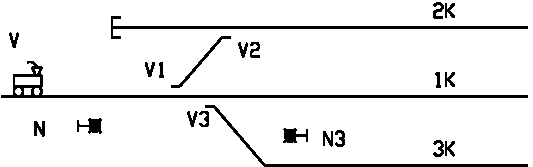
\includegraphics[width=0.8\linewidth]{zzt_fig001.pdf}
    \caption{Stanice
             (\cite[s.~5]{Chudacek2005})}
    \label{zzt:fig001}
  \end{figure}
 
  Před stanicí je umístěno návěstidlo \(N\), které v základní poloze ukazuje návěst \uv{stůj}. Dokud
  návěstidlo ukazuje tuto návěst, nesmí vlak \(V\) do stanice vjet. Má-li vlak vjet bezpečně např. 
  na kolej \(1K\), je třeba splnit určité podmínky. Výměny - pohyblivé části výhybek - \(V1\) a 
  \(V3\) musí být v poloze umožňující řádnou jízdu na kolej \(1K\), tj. jeden jazyk musí
  vždy přiléhat k příslušné opornici, druhý musí být od své opornice náležitě vzdálen. Na koleji 
  \(1K\) (včetně výhybek \(V1\) a \(V3\)) nesmí být žádná vozidla a ani nesmí být povolen příjezd
  jiných vozidel na tuto kolej z opačného směru. Zamýšlenou cestu nesmí ohrožovat z boku pohyby 
  jiných vlaků nebo posunujících dílů, proto výměna \(V2\) musí kolizní jízdu svou polohou 
  znemožňovat a návěstidlo \(N3\) musí kolizní jízdu zakazovat (ochrana odvratnou polohou výměny se 
  nazývá \emph{přímou boční ochranou}, ochrana návěstidlem se zakazující návěstí je \emph{nepřímou 
  boční ochranou}). Když tedy byly všechny prvky zvolené cesty správně nastaveny, přezkoušeny a 
  shledány bez závady, může být návěstidlo \(N\) přestaveno do polohy dovolující jízdu. Po celou 
  dobu, kdy návěstidlo dovoluje jízdu, bude dohlíženo, že všechny k tomu rozhodující podmínky jsou 
  nadále splněny. Vlak \(V\) vjede do stanice a ihned po jeho vjezdu se návěstidlo \(N\) přestaví 
  opět do základní polohy (návěst "stůj"), aby týž povel návěstidla nemohl být využit více vlaky a 
  aby shora uvedený postup bylo třeba pro každý vlak znovu opakovat.

  \begin{figure}[ht!] %\ref{zzt:fig002}
    \centering
    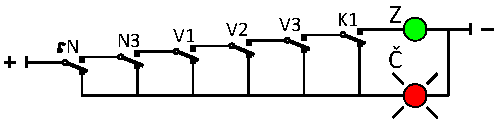
\includegraphics[width=0.8\linewidth]{zzt_fig002.pdf}
    \caption{Vybavení koleje technickým zařízením, které dohlíží na aby vlak vjel do stanice 
             bezpečně
             (\cite[s.~5]{Chudacek2005})}
    \label{zzt:fig002}
  \end{figure}
  
  Úkony, potřebné k tomu, aby vlak vjel do stanice bezpečně, může vykonat určený zaměstnanec. Ten
  se například pochůzkou přesvědčí, že kolej \(1K\) je volná, že výměny jsou řádně postaveny atd. a 
  po ověření všech podmínek přestaví návěstidlo \(N\) do polohy povolující jízdu. Pokud se 
  zaměstnanec nezmýlí, nedojde k nehodě (povšimněme si, že negace této věty nemusí být pravdivá). 
  Bezpečnost jízdy vlaku bude tedy závislá na osobních vlastnostech člověka. Aby tomu tak nebylo, 
  vybavíme koleje technickým zařízením, které bude na jejich volnost dohlížet, výměny jinými
  technickými zařízeními, která budou kontrolovat jejich polohu atd. a jízdní návěst návěstidel
  učiníme nuceně závislou na informacích těchto technických zařízení. Primitivní schéma
  takového zařízení je na obr. \ref{zzt:fig002}. I když pak dopravní zaměstnanec dá návěstním 
  řadičem \(N\) pokyn k rozsvícení jízdní (tj. jízdu povolující) návěsti \(Z\), návěst se rozsvítí 
  jen v případě, že kontakt \(N3\) informuje svým sepnutím, že návěstidlo \(N3\) skutečně ukazuje 
  návěst "stůj", kontakty \(V1\), \(V2\) a \(V3\) informují, že výměny jsou ve správné poloze a 
  kontakt \(K1\) informuje, že první kolej je volná a není na ni postavena jiná cesta. Jízdní 
  návěst \(Z\) se tedy rozsvítí až po splnění všech předem stanovených podmínek pro bezpečný vjezd 
  vlaku. Není-li kterákoliv podmínka splněna, na návěstidle \(N\) zůstává svítit červené světlo Č. 
  
  Přesto takové zařízení \textbf{nelze} považovat za zabezpečovací zařízení. Prvním důvodem je, že 
  nebyly zřízeny \emph{vzájemné závislosti}. Jízdní návěst na návěstidle \(N\) se sice rozsvítí až 
  když jsou splněny všechny podmínky, ale výměny a návěstidla zůstala volná. Nic nebrání, aby se 
  např. poloha výměn změnila dříve, než vlak \(V\) ukončí svou jízdu. Zhasnutí jízdního znaku \(Z\) 
  na návěstidle \(N\) v důsledku ztráty kontroly při přestavení výměny už nemusí být nic platné, 
  protože vlak již mohl návěstidlo minout nebo již není schopen včas zastavit. Nepostačí ale ani 
  zřízení vzájemné závislosti tím, že by rozsvícená jízdní návěst \(Z\) uzavírala výměny a 
  návěstidla v žádoucí poloze (např. prostřednictvím sériově řazeného relé). Vzhledem k nebezpečí
  přerušení sekvence postupných kroků je důležité, aby uzavření výměn a návěstidel bylo provedeno 
  dříve, než se rozsvítí jízdní návěst. Postup stavění jízdní cesty, vyhovující požadavkům 
  zabezpečovací techniky, bude tedy v naznačeném příkladě následující:
  \begin{itemize}\addtolength{\itemsep}{-0.5\baselineskip}
    \item nejprve se přestaví výměny do žádané polohy,
    \item v druhém úkonu (nazývaném závěr jízdní cesty) se při uzavírání výměn a návěstidel 
          přezkouší jejich správná poloha a tedy, že první úkon byl řádně proveden. Pokud první 
          úkon nebyl proveden správně, musí být znemožněn úkon druhý,
    \item obdobně třetí úkon, tj. rozsvícení jízdní návěsti na návěstidle \(N\), je možný jen 
          tehdy, byl-li druhý úkon (a tedy i první úkon) řádně proveden. 
  \end{itemize}
  
  Tím jsme dosáhli požadované \emph{vzájemné závislosti}, jejíž popsaná úroveň je \textbf{prvním
  charakteristickým rysem} zabezpečovacího zařízení. Zařízení z obr. \ref{zzt:fig002} bude podmínce 
  vyhovovat například v případě, že návěstní přepínač \(N\) bude konstrukčně upraven tak, že ho 
  nebude možné přeložit bez provedení \textbf{závěru jízdní cesty}. Důsledkem zavedení závěru 
  jízdní cesty bude potřeba po vlaku jízdní cestu vybavit, tj. závěr zrušit, aby bylo možné s 
  jednotlivými prvky opět volně manipulovat. 

  Ani nyní však ještě nelze v uvedeném příkladě hovořit o zabezpečovacím zařízení. Zařízení musí
  být konstruováno tak, aby \emph{bezpečnost byla zachována i při jakékoliv možné poruše vlastního 
  zařízení}. Tento  požadavek platí jak pro jednotlivé části, tak pro celek a je \textbf{druhým 
  charakteristickým rysem} železniční zabezpečovací techniky. V uvedeném případě to znamená, že 
  zařízení pro kontrolu volnosti koleje nesmí ani při poruše hlásit obsazenou kolej jako volnou, 
  zařízení pro kontrolu polohy výměny nesmí ani při poruše hlásit nesprávně postavenou výměnu jako 
  výměnu správně postavenou, ke zrušení závěru jízdní cesty nesmí ani poruchou dojít dříve než vlak 
  dotčené prvky skutečně mine atd. Právě tak vlastní zapojení pro rozsvícení jízdní návěsti musí 
  být konstruováno tak, aby se jízdní návěst nemohla poruchou zapojení rozsvítit, pokud všechny 
  podmínky pro její svícení nebudou splněny. Jak patrno, vychází se ze základního železničního
  bezpečnostního předpokladu, že zastavení vlaku poskytuje nejvyšší bezpečnost. Tento předpoklad se 
  zásadně liší od principů aplikovaných v letecké dopravě, kosmonautice, nukleární technice, 
  navigaci, řízení procesů, robotice, dolování, systémech zabezpečení proti vloupání či odcizení 
  atd., kde je prozatím obvykle hlavním cílem dosažení maximální spolehlivosti a pohotovosti 
  systému.
  
  Důsledkem druhého charakteristického rysu zabezpečovací techniky, tj. převedení všech poruch
  bezpečnějším směrem je, že téměř každá porucha zabezpečovacího zařízení znamená omezení dopravy. 
  To samozřejmě může vést k narušení plynulosti a vzniku provozních nepravidelností, což jsou jevy, 
  které samy o sobě nebezpečí v dopravě výrazně zvětšují. Ve vážnějších případech je nutné 
  zabezpečovací zařízení do skončení jeho opravy zcela vypnout, aby byl možný alespoň omezený pohyb 
  vlaků. Pak se ovšem provoz, jehož pravidelnost je navíc narušena, děje bez jakékoliv podpory 
  zabezpečovacího zařízení, zatížen, byť i jen na omezenou dobu, možnými lidskými omyly. Odtud tedy 
  plyne třetí charakteristický rys zabezpečovací techniky, což je taková konstrukce zařízení, která 
  má co nejméně poruch, tedy vysokou spolehlivost nebo - obecněji - co nejvyšší pohotovost. 
 
  Úloha zabezpečovací techniky nekončí zajištěním odpovídajícího návěstního znaku na návěstidle.
  Také na lokomotivě je strojvedoucí, jemuž je svěřena péče o bezpečnost vlaku a který tuto 
  bezpečnost může ohrozit svým omylem. Působnost zabezpečovacích zařízení se tedy (prostřednictvím 
  vlakového zabezpečovacího zařízení) prodlužuje až na vozidlo, aby se zajistilo, že vlak také 
  skutečně bude návěsti respektovat. 

  Aplikují-li se všechny výše uvedené zvláštnosti správně při vývoji zabezpečovacího systému, je
  třeba se postarat také o to, aby nedošlo k jejich znehodnocení při projekci, výrobě, montáži a 
  údržbě konkrétních zařízení. Při těchto činnostech je také třeba počítat s lidskými vlastnostmi. 
  Zařízení, sloužící primárně pro eliminaci chyb dopravních zaměstnanců konstruují, vyrábějí, 
  montují a udržují opět lidé. Naštěstí tyto práce, na rozdíl od výkonu dopravní služby, probíhají 
  (nebo by rozhodně měly probíhat) v lepších podmínkách a bez časové tísně. Za příznivých podmínek 
  se nedokonalosti člověka tolik neuplatňují a práci každého pracovníka lze kontrolovat jinými s 
  případnou pomocí dalších technických zařízení. Přesto však z toho pro projekci, výrobu, montáž a 
  údržbu zabezpečovacích zařízení vyplývají jisté zvláštnosti. 
  
  Vedle úloh z oblasti bezpečnosti plní moderní zabezpečovací technika i úkoly další. Především jde
  o hlubší zásahy do vlastního provozu prostředky automatizace. Ta pak, při správném provedení, 
  vede k zlepšenému využití technických prostředků železnic (např. zvýšení propustné výkonnosti 
  tratí), k zhospodárnění provozu, k úspoře jiných, podstatně vyšších investičních nákladů (např. 
  budování další koleje). Protože však zabezpečovací zařízení je zařízením v zásadě restriktivním, 
  nelze u něj bezhlavě prosazovat zvyšování výkonnosti vždy a ve všech směrech. Později také 
  uvidíme, že zabezpečovací technika se podílí na zvyšování bezpečnosti i v jiných oblastech: 
  kolejové obvody alespoň částečně dohlíží na stav jízdní dráhy (celistvost kolejnic), přestavná 
  zařízení výměn dohlíží na stav výhybek, vlakové zabezpečovače mohou do určité míry dohlížet na 
  stav brzdové soustavy vlaku (sledováním skutečně dosaženého odrychlení při brzdění), přejezdová 
  zabezpečovací zařízení se podílejí na eliminaci cizích vlivů na dopravu atd.
  
  Souhrnně lze konstatovat, že prvořadým účelem zabezpečovacích zařízení na železnici je
  předcházet kolizím a vykolejení vlaků z důvodu chybného řízení dopravy. K tomu účelu je u 
  zařízení třeba sledovat následující oblasti:
  \begin{itemize}\addtolength{\itemsep}{-0.5\baselineskip}
    \item funkční bezpečnost (korektnost systému), tj. řádné plnění všech požadovaných funkcí v 
          bezporuchovém stavu a při očekávaných vlivech pracovního prostředí,
    \item technickou bezpečnost (bezpečnou konstrukci), tj. splnění požadavku, aby nedošlo k 
          přímému ohrožení bezpečnosti dopravy ani při poruchách samotného zabezpečovacího zařízení,
    \item bezpečnou aplikaci, tj. vytvoření takových logických funkcí a vzájemných závislostí, aby 
          pro konkrétní situaci navržené zařízení ve všech provozních stavech mohlo řádně plnit 
          svou funkci (na jeho výstupech budou jízdu povolující informace pouze v takovém rozsahu, 
          který odpovídá stavu informací vstupních) a zajištění, aby tyto vlastnosti zařízení mělo 
          i po výrobě a montáži,
    \item bezpečný provoz a údržbu, tj. zajištění, že předchozí úrovně zůstanou v zařízení 
          zachovány po celou dobu životnosti,
    \item vysokou spolehlivost, tj. omezení případů, kdy nepřímo, vyřazením zabezpečovacího 
          zařízení a přechodem na manuální řízení, by mohlo dojít k ohrožení bezpečnosti dopravy.
  \end{itemize}
  Žádnou ze zmíněných oblastí nelze preferovat, protože žádná nemůže nahradit druhou a             
  nedostatky v kterékoliv z nich znehodnocují výsledky ostatních.
  
  Přímým obsahem železniční zabezpečovací techniky není zajištění zdraví a bezpečnosti
  zaměstnanců (i když provozovaná zařízení samozřejmě musí splňovat i požadavky např. ve směru 
  ochrany před nebezpečným dotykovým napětím, ergonomicky správně navrženého obsluhovací pracoviště 
  atd.), zabránit nehodám ze zlého úmyslu, násilnou obsluhou, úmyslným poškozením nebo zneužitím 
  zařízení. V poslední době se však jeví jako nezbytné dokonaleji zajišťovat zabezpečovací zařízení 
  proti vandalům a lapkům všeho druhu a neoprávněným zásahům do zařízení v případě, že používají 
  jiných než speciálně drážních zařízení (viz dále např. ochrana dat v otevřených sítích).  

\section{Třídění}
  K železničním zabezpečovacím zařízením se obvykle řadí i zabezpečovací zařízení používaná na
  podzemních drahách (metro, doly), na pouličních drahách (tramvaje - zejména městské rychlodráhy) 
  a na vlečkách, protože využívají obdobných principů, často i obdobná nebo jen poněkud upravená 
  zařízení. Při třídění zařízení lze použít řadu třídících hledisek; téměř vždy se však vyskytnou 
  zařízení přechodová (smíšená) nebo podle užitého třídění obtížně definovatelná. Přesto je dále 
  několik třídění uvedeno, protože poskytují obrázek o pestrosti a mnohotvárnosti pojednávaného 
  zařízení. 
  
  Nejpřirozenějším a klasickým tříděním zabezpečovacích zařízení je třídění podle účelu zařízení.
  Podle tohoto hlediska lze zabezpečovací zařízení dělit na zařízení: 
  \begin{itemize}\addtolength{\itemsep}{-0.5\baselineskip}
    \item staniční,
    \item traťové,
    \item vlakové,
    \item přejezdové, 
    \item spádovištní. 
  \end{itemize}
  Účel je patrný již z názvu. Staniční zabezpečovací zařízení zajišťuje bezpečný pohyb vlaků ve 
  stanici, traťové zařízení zabezpečuje jízdu vlaku na trati mezi stanicemi, vlakové zařízení 
  zabraňuje vlaku pohybovat se nad rámec, který povoluje zařízení staniční a traťové (s případným 
  zahrnutím i dalších omezení), přejezdové zařízení přispívá k zajištění bezpečnosti na úrovňovém 
  křížení silnice a železnice informováním uživatelů silnice, že se k přejezdu blíží vlak s 
  předností v jízdě. Nad všemi těmito zařízeními pak může být budováno zařízení pro dálkové 
  ovládání většího úseku tratě z jednoho místa. 
  
  Podle místa ovládání zařízení mluvíme o zařízení s obsluhou :
    \begin{itemize}\addtolength{\itemsep}{-0.5\baselineskip}
    \item místní,
    \item ústřední (centralizovanou v oblasti jedné stanice),
    \item dálkovou (mimo vlastní stanici).
  \end{itemize}

  Další třídění je odvozeno od způsobu ovládání periferií (výměn, návěstidel atd.) a tak vlastně
  zahrnuje celou historii železniční zabezpečovací techniky. Rozeznáváme zařízení:
  \begin{itemize}\addtolength{\itemsep}{-0.5\baselineskip}
    \item mechanická (využívající výhradně lidské síly),
    \item elektrická,
    \item pneumatická,
    \item hydraulická. 
  \end{itemize}

  Obdobně, v následujícím třídění je rozhodující způsob, jímž se v zařízení potřebné závislosti
  realizují. Zde rozeznáváme zařízení se závislostmi:
  \begin{itemize}\addtolength{\itemsep}{-0.5\baselineskip}
    \item mechanickými,
    \item mechanickými i elektrickými (tzv. elektromechanická a elektrodynamická zařízení),
    \item elektrickými, která lze dále dělit podle rozhodujících stavebních prvků, jimiž jsou 
         závislosti realizovány, na zařízení:
       \begin{itemize}
       \item reléová,
       \item hybridní (rozhodující část bezpečné logiky je realizována reléově, zbytek 
             elektronicky),
       \item elektronická (mikroprocesorová). 
       \end{itemize}
  \end{itemize}

  U traťových zabezpečovacích zařízení je kladen důraz na rozsah spolupůsobení vlaku. Zařízení se
  pak dělí na:
  \begin{itemize}\addtolength{\itemsep}{-0.5\baselineskip}
    \item poloautomatická (poloautobloky),
    \item automatická (autobloky).
  \end{itemize}
  Podle rozmístění traťových zařízení podél trati lze automatická zařízení dále dělit na:
  \begin{itemize}\addtolength{\itemsep}{-0.5\baselineskip}
    \item decentralizovaná (funkční bloky jsou umístěny v každém návěstním bodě),
    \item částečně centralizovaná (funkční bloky jsou umístěny pouze ve vybraných bodech na trati),
    \item centralizovaná (zařízení je koncentrováno do stanic).
  \end{itemize}
  Vlaková zabezpečovací zařízení se dělí podle způsobu přenosu informací mezi tratí a hnacím
  vozidlem na zařízení:
  \begin{itemize}\addtolength{\itemsep}{-0.5\baselineskip}
    \item bodová,
    \item semiliniová,
    \item liniová. 
  \end{itemize}

  Podle způsobu kontroly souladu jízdy vlaku s přenášenými informacemi se vlaková zařízení dále 
  dělí na zařízení s kontrolou:
  \begin{itemize}\addtolength{\itemsep}{-0.5\baselineskip}
    \item bdělosti strojvedoucího,
    \item rychlosti vlaku.
  \end{itemize}
  
  Zařízení přejezdová se dělí podle způsobu výstrahy na přejezdová zařízení:
  \begin{itemize}\addtolength{\itemsep}{-0.5\baselineskip}
    \item mechanická,
    \item světelná bez závor,
    \item světelná se závorami.
  \end{itemize}
  
  U moderních systémů dělení zabezpečovacích zařízení na zařízení staniční, traťová, vlaková a
  přejezdová ztrácí smysl, protože systémy jsou komplexní, se společným jádrem řídícím jednotlivé 
  periférie a tyto celky pak tvoří nanejvýš podsystémy. Na obr. 3-1 je základní blokové schéma 
  takového systému. 
  \begin{figure}[ht!] %\ref{zzt:fig003}
    \centering
    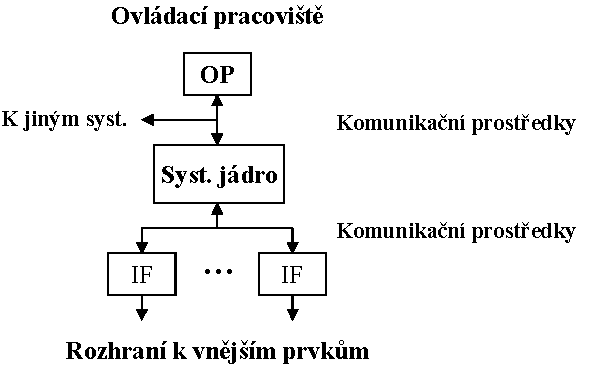
\includegraphics[width=0.8\linewidth]{zzt_fig003.pdf}
    \caption{Stanice
             (\cite[s.~11]{Chudacek2005})}
    \label{zzt:fig003}
  \end{figure}


  \section{Klasifikace poruch}
    \textbf{Chyba} je rozdíl mezi správnou a skutečnou hodnotou nějaké veličiny. V zařízení se 
    chyby mohou obecně objevit jako \emph{důsledek (projev) poruchy některé jeho součásti, 
    působením nějakého cizího vlivu} nebo \emph{selháním lidského činitele}. Za poruchy hardware se 
    považují všechna vybočení z předpokládaných vlastností stavebního prvku (součástky, dílu) 
    zařízení. Předpokládanými vlastnostmi prvků přitom jsou vlastnosti odpovídající příslušným 
    technickým podmínkám popisujícím jeho vlastnosti. Jako omyl lze označit každou lidskou činnost, 
    která může vést k nezamýšlenému chování zařízení. V širším slova smyslu se jako 
    \textbf{porucha} označují souhrnně všechny příčiny vedoucí k chybě, tj. poruch součásti, 
    cizí vliv i omyl.

%~~~~~~~~~~~~~~~~~~~~~~~~~~~~~~~~~~~~~~~~~~~~~~~~~~~~~~~~~~~~~~~~~~~~~~~~~~~~~~~~~~~~~~~~~~~~~~~~~~
\printbibliography[title={Seznam literatury}, heading=subbibliography]
\addcontentsline{toc}{section}{Seznam literatury}

\chapter{Bezpečnost a spolehlivost zabezpečovacích systémů}
 \section{Spolehlivost}
 \section{Bezpečnost}
    V různých publikacích je možné najít různé definice bezpečnosti. Například norma 
    EN~61508\footnote{Funkční bezpečnost elektrických/elektronických/programovatelných 
    elektronických systémů souvisejících s bezpečností (Functional safety of electrical/ 
    electronic/programmable electronic systems), obecná norma funkční bezpečnosti, která se opírá o 
    dvě základní koncepce - životní cyklus bezpečnosti a úroveň integrity bezpečnosti 
    (\texttt{SIL})} 
    definuje bezpečnost jako nepřítomnost netolerovaného rizika. Z této definice je zřejmé, že 
    bezpečnost je úzce spjatá s rizikem, a je nutné bezpečnost třeba chápat relativně. Když se 
    řekne, že řídicí systém je bezpečný, neznamená to jeho absolutní bezpečnost (ta je prakticky 
    nedosažitelná vzhledem na existenci objektivních faktorů, jako je například úroveň poznání, 
    technologická úroveň a limitované finanční prostředky), ale taková úroveň bezpečnosti, 
    která zodpovídá definovaným bezpečnostním požadavkům na tento řídicí systém. 

    Relativnost v pojímání bezpečnosti znamená posun od kvalitativního ke kvantitativnímu chápaní bezpečnosti.

    Kvalitativně je bezpečnost chápána jako schopnost řídicího systému zajistit omezení důsledků 
    poruch řídicích systému v daných podmínkách a v daném časovém intervalu. Matematicky je možné 
    kvalitativní bezpečnost řídicího systému vyjádřit jako 
    \begin{equation}
      E_H = 0,
    \end{equation}
    kde \(E_H\) je množina nebezpečných stavů, které jsou důsledkem výskytu pravděpodobných poruch 
    řídicího systému. Pravděpodobná porucha je taková porucha z množiny všech poruch, jejichž 
    výskyt během provozu řídicího systému je nutné předpokládat (vzhledem na požadovanou úroveň 
    bezpečnosti řídicího systému).
	
    Kvantitativně je bezpečnost řídicího systému chápána jako pravděpodobnost nepřítomnosti
    jakéhokoliv nebezpečného stavu v řídicím systému v daných podmínkách a v daném časovém
    intervalu. Je zřejmé, že i když pravděpodobnost nebezpečného stavu řídicího je malá, neznamená
    to, že se nebezpečný stav nemůže vyskytnou v nejbližším časovém intervalu, Matematicky je možné
    kvantitativní bezpečnost vyjádřit tak, že
    \begin{equation}
      P_{HT}(t)\geq P_{HT}(t)>0,
    \end{equation}
    kde \(P_{HT}(t)\) je pravděpodobnost tolerovaného nebezpeční řídicího systému a \(P_{HR}(t)\)
    je reálná pravděpodobnost nebezpeč\-ného stavu řídicího systému.
	 
    Na kvantitativním hodnocení bezpečnosti řídicího systému je v podstatě možné uplatnit stejné 
    teoretické postupy, jako při hodnocení spolehlivosti technických systémů. Zásadní rozdíl je v 
    tom, že při hodnocení spolehlivosti standardních řídicích systémů se obvykle rozlišují dva 
    stavy - bezporuchový stav a poruchový stav, a k těmto dvěma stavům se vztahují také 
    kvantitativní ukazatele spolehlivosti. Při hodnocení bezpečnosti řídicích systémů musíme 
    uvažovat s dvěma druhy poruchových stavů - bezpečným a nebezpečným poruchovým stavem. 
    Bezpečnost řídicího systému se potom vyjadřuje pomocí ukazatelů bezpečnosti (například 
    pravděpodobnost výskytu nebezpečné poruchy, intenzita nebezpečných poruch, ...).

    Při kvantitativním hodnocení důsledků poruch na bezpečnost řídicího systému se obvykle k 
    hodnoceným řídicím systémům přistupuje jako k neobnovovaným objektům, protože z pohledu 
    bezpečnosti jsou důležité dva stavy (bezpečný, nebezpečný) a analýza končí výskytem nebezpečné 
    poruchy (může jít o jednu poruchu, nebo o kombinaci více poruch, které nejsou individuálně 
    nebezpečné). To znamená, že od uvedení řídicího systému do provozu, až po výskyt nebezpečné 
    poruchy, se může řídicí systém střídavě nacházet ve funkčním, nebo nefunkčním stavu (nefunkční 
    ještě neznamená nebezpečný). Z tohoto důvodu ukazatele bezpečnosti jsou podobné ukazatelům 
    bezporuchovosti neobnovovaných objektů. 
  
    \subsection{Základní legislativa}
      \begin{itemize}
        \item \textbf{EN 61508} - \emph{základní všeobecná norma pro SRCS}; pojednává o funkční
              bezpečnosti elektrických/elektronických/programovatelných elektronických systémů
              souvisejících s bezpečností (Functional safety of electrical/electronic/programmable
              electronic systems), obecná norma funkční bezpečnosti, která se opírá o dvě základní
              koncepce - životní cyklus bezpečnosti a úroveň integrity bezpečnosti (\texttt{SIL})
              \begin{itemize}
                \item EN 61508-1: Všeobecné požadavky
                \item EN 61508-2: Požadavky na elektrické / elektronické / programovatelné
                                  elektronické systémy související s bezpečností
                \item EN 61508-3: Požadavky na SW
                \item EN 61508-4: Definice a zkratky
                \item EN 61508-5: Příklady metod určování úrovně integrity bezpečnosti
                \item EN 61508-6: Metodické pokyny na používání EN 61508-2, STN EN 61508-3
                \item EN 61508-7: Přehled technik a opatření
              \end{itemize}
        \item \textbf{EN 50126}: Railway applications – The specification and demonstration of
              reliability, availability, maintainability and safety (RAMS)
              \begin{itemize}
                \item Part 1: Basic requirements and generic process. 1999
                \item Part 2: Guide to the application of EN 50126-1 for safety. 2007
                \item Part 3: Guide to the application of EN 50126-1 for rolling stock RAMS. 2008  
              \end{itemize}
              Zabývá se specifikací parametrů RAMS (spolehlivost, pohotovost, udržovatelnost,
              a bezpečnost) obecně pro všechny železniční systémy, reaguje na skutečnost, že
              naléhavost požadavků na bezpečnost funkce jednotlivých železničních systémů je různá
              a lze je tedy splňovat s různou pravděpodobností jejich selhání. Také zavádí pojem
              \emph{integrita bezpečnosti (safety integrity - celistvost, úplnost, neporušenost
              bezpečnosti)}, který definuje jako pravděpodobnost, s níž systém uspokojivě splní
              požadované bezpečnostní funkce, za všech stanovených podmínek a ve stanoveném časovém
              období. Jde o to, do jaké míry může být pro bezpečnost relevantní funkce narušena
              např. poruchami vlastního zařízení, omyly obsluhy, vnějším rušením atd.
        \item \textbf{EN 50128}: Railway applications – Communication, signalling and processing
              systems – Software for railway control and protection systems. 2003          
        \item \textbf{EN 50129}: Railway applications – Communication, signalling and processing
              systems – Safety-related electronic systems for signalling. 2011
              Modifikovaně byl pojem integrita bezpečnosti přenesen i do této normy pro železniční
              zabezpečovací systémy. I klasická zabezpečovací technika bez velkého zdůrazňování
              respektovala, že nejsou na všechna zařízení kladeny stejně důrazné bezpečnostní
              požadavky (kategorie zařízení, vedlejší tratě/hlavní tratě, zařízení pro ČD/zařízení
              pro vlečky, staniční zařízení/spádoviště atd.). Uvidíme dále, že pojmu integrita
              bezpečnosti je pro zabezpečovací zařízení dominantně obsažena oblast, kterou běžně v
              této technice označujeme(a také normá EN 50129 ji tak označuje ve své základní části)
              termínem technická bezpečnost. Úvahy okolo integrity bezpečnosti zde sledujeme
              odděleně od úvah o technické bezpečnosti (přes jejich podobnost) pro jejich výhodnost
              zejména v úvodních fázích projektu nového systému (zařízení, výrobku, atd.)
        \item \textbf{EN 50159: Railway applications – Communication, signalling and processing
              systems - Safety-related communication in transmission systems. 2010}            
      \end{itemize}
    
      Vyjmenované normy se poněkud liší v definici termínu \emph{bezpečnost}:  
      \begin{itemize}
        \item Bezpečnost (Safety) – nepřítomnost nepřijatelných úrovní rizika poškození (EN50129)
        \item Bezpečnost (Safety) – nepřítomnost nepřijatelného rizika. (EN61508)
        \item Bezpečnost při poruše (Fail Safe) – vlastnost konstrukce objektu zabraňující,
              aby jeho poruchy způsobili nebezpečné poruchové stavy. (IEC 50 (191))
        \item Kvalitativní bezpečnost – schopnost systému zajistit omezení důsledku poruch
              systému v daných podmínkách a v daném časovém intervale.
        \item Kvantitativní bezpečnost – pravděpodobnost nepřítomnosti jakéhokoliv
              nebezpečného stavu v systéme v daných podmínkách a v daném časovém intervale.
      \end{itemize}

    \subsection{Ukazatel bezpečnosti}
      \fbox{Pravděpodobnost bezpečného provozu} je pravděpodobnost, že objekt může bezpečně plnit 
      požadovanou funkci v daných podmínkách v časovém intervalu \(t_1,\, t_2\).
      \begin{equation}
        R_S(t_1,\, t_2) = 1- F_H(t_1,\, t_2),
      \end{equation}
      kde \(F_H(t_1,\, t_2)\) je distribuční funkce, která naopak vyjadřuje pravděpodobnost, že
      objekt nemůže bezpečně plnit požadovanou funkci k daným podmínkám v časovém intervalu
      \(t_1,\, t_2\).
      \begin{equation}
        F_H(t_1,\, t_2) = \int_{t_1}^{t_2}f_H(t)\cdot\dd{t},
      \end{equation}
      kde \(f_H(t)\) je hustota pravděpodobnosti nebezpečné poruchy objektu. 

      \fbox{Intenzita nebezpečných poruch} \(\lambda_H(t)\) definujme jako limitu poměru podmíněné
      pravděpodobnosti, že časový okamžik vzniku nebezpečné poruchy objektu \(T\) padne do daného
      časového intervalu \(t,\, t+\Delta t\), přičemž délka časového intervalu \(\Delta
      t\rightarrow0\)
      \begin{equation}\label{DZT:eq_def_lambdaH}
        \lambda_H=\frac{f_H(t)}{R_S(t)}.
      \end{equation}

      Protože nebezpečné poruchy jsou méně časté, zkoušky na určení požadovaných ukazatelů
      bezpečnosti by bylo třeba provádět dlouhodobě, což je prakticky nemožné. 
    
  \section{Integrita bezpečnosti}
    Všeobecně je možné konstatovat, že SRCS realizuje řídící i ochranné funkce (obr.
    \ref{DZT:fig_DZT_SRCS_fce}). Jelikož selhání řídicí funkce může způsobit ohrožení bezpečnosti,
    je třeba i tyto funkce považovat za bezpečnostní.
    \begin{figure}[hb!]
      \centering
      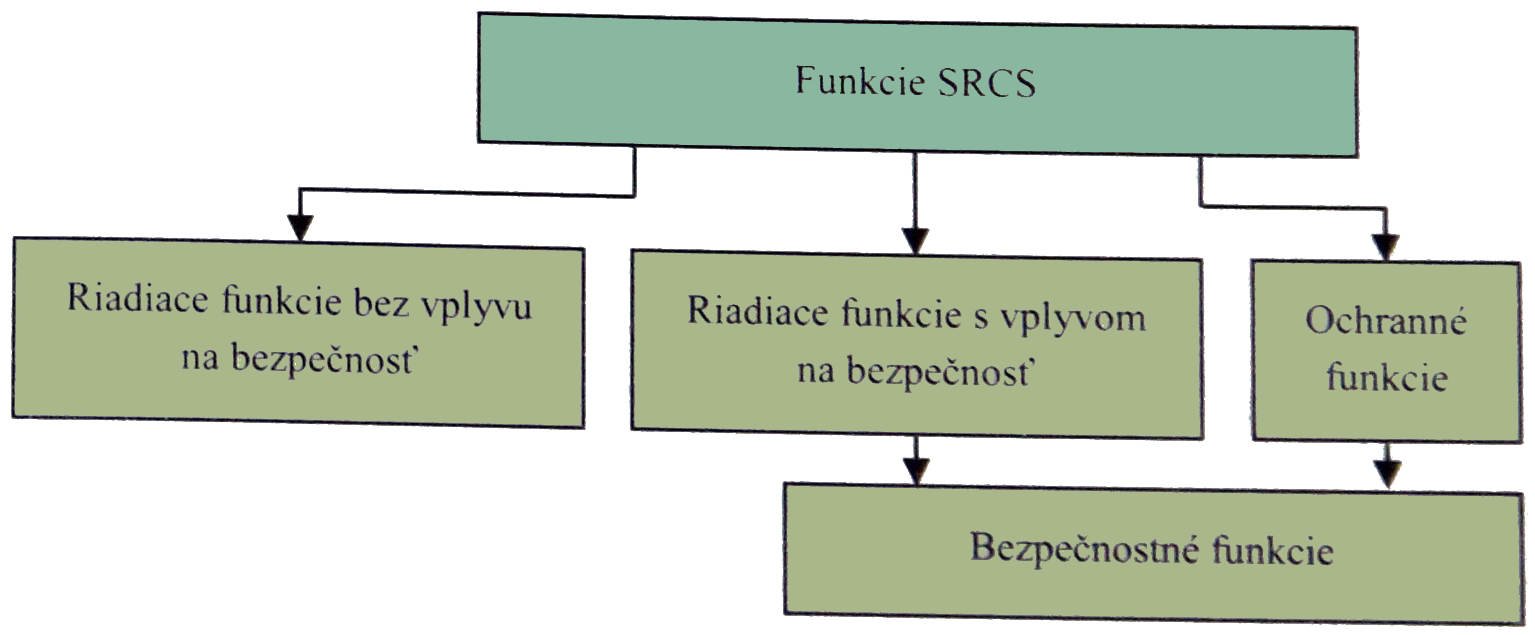
\includegraphics[width=1\linewidth]{DZT_SRCS_fce.jpg}
      \caption{Vztah mezi bezpečnostními funkcemi a moduly SRCS}
      \label{DZT:fig_DZT_SRCS_fce}
    \end{figure}    
    Bezpečnostní funkce jsou definované na základě analýzy rizik jako technická opatření na snížení
    rizika spojeného s konkrétními nebezpečí na tolerovatelnou úroveň. Účinnost bezpečnostní funkce
    se určuje pomocí úrovně integrity bezpečnosti \emph{(\texttt{SIL} - safety integrity level)}. 
    
    Norma \emph{EN 61508} definuje integritu bezpečnosti jako pravděpodobnost, že SRCS bude plnit 
    požadované bezpečné funkce za všech stanovených podmínek v rámci stanoveného operačního 
    prostředí a během stanoveného časového období. Všeobecně lze konstatovat, že čím je integrita
    bezpečnosti SRCS větší, tím je menší pravděpodobnost selhání bezpečností funkce realizovaných
    SRCS.  
    
    Integrita bezpečnosti se skládá ze dvou částí a to:
    \begin{itemize}
      \item \emph{integrity bezpečnosti proti systematickým poruchám}: jde o nekvantifikovatelnou
            část integrity bezpečnosti, která souvisí s nebezpečnými systematickými poruchami 
            hardware a software; integrity bezpečnosti proti systematickým poruchám se dosahuje
            především opatřeními na předcházení chybám a poruchám; vzhledem k tomu, že jde o 
            nekvantifikovatelnou část integrity bezpečnosti, je vhodnější chápat integritu 
            bezpečnosti jako vlastnost a né jako pravděpodobnost; hodnocení integrity bezpečnosti
            proti systematickým chybám a poruchám se realizuje kontrolou dodržování opatření
            předcházejících chybám a poruchám, mezi které patří také důsledné testování korektní
            realizace bezpečnostních funkcí; 
      \item \emph{integrity bezpečnosti proti náhodným poruchám}: jde o kvantifikovatelnou část
            integrity bezpečnosti, která se týká náhodných poruch hardware vyplývajících z konečné
            bezporuchovosti použitých součástek; hodnocení integrity bezpečnosti proti náhodným
            poruchám se realizuje prostřednictvím pravděpodobnostních výpočtů.
    \end{itemize}
    
    Aby se dosáhla požadovaná integrita bezpečnosti, musí být splněné požadavky na integritu proti 
    systematickým poruchám i náhodným poruchám. 
    
    \subsection{Úroveň integrity bezpečnosti}
      Úroveň integrity bezpečnosti (\emph{Safety Integrity Levels - \texttt{SIL}}) se dělí podle EN 
      50129
      do čtyř kategorií - úroveň 4 (\texttt{SIL} 4) je nejvyšší, úroveň 1 (\texttt{SIL} 1) je 
      nejnižší.  Pokud se
      objevuje úroveň \texttt{SIL} 0, značí to, že se jedná o systém na které nejsou kladeny žádné
      bezpečnostní požadavky (ve smyslu zabezpečovací techniky)
      
      Proto, aby SRCS mohl být zařazen do odpovídající úrovně bezpečnosti \texttt{SIL}, musí 
      vyhovovat
      těmto faktorům:
      \begin{itemize}
        \item naplnění podmínek řízení kvality, 
        \item naplnění podmínek řízené bezpečnosti,
        \item splnění požadavků na technickou bezpečnost, 
        \item dosažení kvantitativního cíle
      \end{itemize}
      
      Jak patrno, splnění kvantitativního ukazatele samo o sobě neznamená, že bylo dosaženo
      odpovídající úrovně bezpečnosti. To platí ovšem i naopak - splnění tří předchozích podmínek
      (řízení kvality, řízení bezpečnosti a technické bezpečnosti) nezaručuje, že bylo dosaženo
      kvantitativních cílů a nelze tedy tvrdit, že zařízení lze zařadit do odpovídající skupiny
      \texttt{SIL} (\ref{DZT:fig_EN50129_SIL_techniques}).
      
      \begin{figure}[ht!]% Relationship between \texttt{SIL}s and techniques
        \centering
        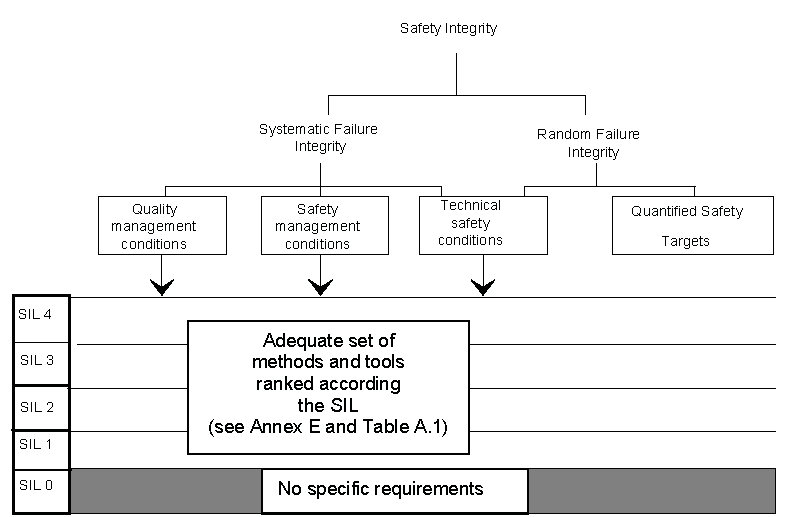
\includegraphics[width=0.95\linewidth]{EN50129_SIL_techniques.pdf}
        \caption{Vztah mezi \texttt{SIL} úrovní a technikami jejich dosažení}
        \label{DZT:fig_EN50129_SIL_techniques}
      \end{figure}
      
      Žádná z norem \texttt{CENELEC} nepředepisuje, které zařízení musí být jaké úrovně. Toto 
      určení je 
      ponecháno na provozovateli, resp. regulátorovi, vyplyne také z provedených analýz rizik 
      a hazardů.
      
      Následující tabulka shrnuje definované úrovně integrity bezpečnosti a zároveň dává do
      souvislosti s tolerovatelnými četnostmi hazardů. \texttt{SIL} jsou tedy prostředkem přiřazení
      kvalitativních přístupů (pro vyloučení systematických poruch) ke kvantitativnímu přístupu
      (pro řízení náhodných poruch), neboť systematické poruchy nelze kvantifikovat.
      \begin{table}[h]
        \centering
        \begin{tabular}{|c|c|}
          \hline
           Úroveň integrity &  Tolerovatelná četnost hazardu            \\
             bezpečnosti \texttt{SIL} &  THR [za hodinu a funkci]       \\ \hline\hline 
              4        & \(10^{-9}\leq THR < 10^{-8}\)                  \\ \hline
              3        & \(10^{-8}\leq THR < 10^{-7}\)                  \\ \hline
              2        & \(10^{-7}\leq THR < 10^{-6}\)                  \\ \hline
              1        & \(10^{-6}\leq THR < 10^{-5}\)                  \\ \hline
        \end{tabular}
        \caption{\texttt{SIL} tabulka: Funkce, jejichž kvantitativní požadavky by převyšovaly 
                 hranici \(10^{-9}\), která se zdánlivě nelogicky objevuje u \texttt{SIL4}, vyžaduje
                 podle normy \texttt{EN~50129} zvláštní technická nebo provozní opatření pro 
                 dosažení tak mimořádného cíle.}
      \end{table}
       
      \begin{enumerate}
        \item Z normy jasně vyplývá rozdělení na dvě skupiny \texttt{SIL 1,2} vs. \texttt{SIL 3,4}, 
              u nichž je výrazný rozdíl v požadavcích, které je potřeba splnit, aby SRCS mohl 
              patřit do dané skupiny. To je velmi dobře patrné z tabulek v příloze \texttt{E} normy 
              \texttt{EN 50129}, která se zabývá technikami a opatřeními pro řízení náhodných a 
              systematických poruch. 
        \item Druhým důležitým faktem je poněkud odlišná definice chápání úrovní \texttt{SIL} v 
              EN~61508. \emph{Funkční bezpečnost elektrických, elektronických, programovatelných
              elektronických systémů souvisejících s bezpečností}. Tato norma je obecnou normou pro
              průmyslové elektronické systémy, z níž vycházejí normy EN~50126, EN 50~129 atd.
              jakožto specifické normy pro železniční aplikace. Důležitou odlišností ve specifikaci
              \texttt{SIL}, viz tab. 2 a 3 v první části této normy (EN~61508-1). Nicméně tabulka 3 
              pro
              režim provozu s vysokým, resp. nepřetržitým vyžádáním odpovídá tabulce v normě
              EN~50129. Avšak i pro tyto systémy se zde jeví určitá odlišnost v požadavcích na
              zajištění dané \texttt{SIL}. Norma EN~61508 je zaměřena pouze na \emph{funkční 
              bezpečnost},
              není zde zahrnutý požadavek na bezpečnou reakci na ojedinělé náhodné poruchy. S
              poruchami se samozřejmě pracuje, mají být provedena opatření k jejich maximálnímu
              potlačení - četnosti i následku, nicméně může stačit, když systém je schopen poruchy
              detekovat a dát o nich vědět (např. obsluze). Závěrem nutno dodat, že je potřeba
              určité obezřetnosti k tvrzení, že systém splňuje daný \texttt{SIL}. Tento údaj musí 
              být
              doplněn specifikací, která norma byla při klasifikaci použita.
      \end{enumerate}
      
%\end{Czech}

%} %tikzset
%~~~~~~~~~~~~~~~~~~~~~~~~~~~~~~~~~~~~~~~~~~~~~~~~~~~~~~~~~~~~~~~~~~~~~~~~~~~~~~~~~~~~~~~~~~~~~~~~~~
\printbibliography[title={Seznam literatury}, heading=subbibliography]
\addcontentsline{toc}{section}{Seznam literatury}
} % DEBUG was off

%==================================================================================================

\part{PZT}\label{part:PZT}
\parttoc

\ifthenelse{ \equal{\DebugMode}{true} }{
% Debug mode ON
  % !TeX spellcheck = cs_CZ
%{\tikzset{external/prefix={tikz/PZT/}}
% \tikzset{external/figure name/.add={ch01_}{}}
%---------------------------------------------------------------------------------------------------
% file ra3ch001.tex
%---------------------------------------------------------------------------------------------------
%====================Kapitola: Výhybky =============================================================
\chapter{Výhybka}\label{pzt:chapI}
\minitoc

%} %tikzset
%~~~~~~~~~~~~~~~~~~~~~~~~~~~~~~~~~~~~~~~~~~~~~~~~~~~~~~~~~~~~~~~~~~~~~~~~~~~~~~~~~~~~~~~~~~~~~~~~~~
\printbibliography[title={Seznam literatury}, heading=subbibliography]
\addcontentsline{toc}{section}{Seznam literatury}

  % !TeX spellcheck = cs_CZ
%{\tikzset{external/prefix={tikz/PZT/}}
% \tikzset{external/figure name/.add={ch02_}{}}
%---------------------------------------------------------------------------------------------------
% file ra3ch001.tex
%---------------------------------------------------------------------------------------------------
%====================Kapitola: Detekce kolejových vozidel ==========================================
\chapter{Detekce kolejových vozidel}\label{pzt:chapII}
\minitoc

%} %tikzset
%~~~~~~~~~~~~~~~~~~~~~~~~~~~~~~~~~~~~~~~~~~~~~~~~~~~~~~~~~~~~~~~~~~~~~~~~~~~~~~~~~~~~~~~~~~~~~~~~~~
\printbibliography[title={Seznam literatury}, heading=subbibliography]
\addcontentsline{toc}{section}{Seznam literatury}

  % !TeX spellcheck = cs_CZ
%{\tikzset{external/prefix={tikz/PZT/}}
% \tikzset{external/figure name/.add={ch03_}{}}
%---------------------------------------------------------------------------------------------------
% file ra3ch001.tex
%---------------------------------------------------------------------------------------------------
%====================Kapitola: Detekce kolejových vozidel ==========================================
\chapter{Návěstidlo}\label{pzt:chapIII}
\minitoc
%} %tikzset
%~~~~~~~~~~~~~~~~~~~~~~~~~~~~~~~~~~~~~~~~~~~~~~~~~~~~~~~~~~~~~~~~~~~~~~~~~~~~~~~~~~~~~~~~~~~~~~~~~~
\printbibliography[title={Seznam literatury}, heading=subbibliography]
\addcontentsline{toc}{section}{Seznam literatury}

}
{
 % DEBUG was off
%========== Kapitola 001: Bezpečnost a spolehlivost zabezpečovacích systémů =======================
  % !TeX spellcheck = cs_CZ
%{\tikzset{external/prefix={tikz/PZT/}}
% \tikzset{external/figure name/.add={ch01_}{}}
%---------------------------------------------------------------------------------------------------
% file ra3ch001.tex
%---------------------------------------------------------------------------------------------------
%====================Kapitola: Výhybky =============================================================
\chapter{Výhybka}\label{pzt:chapI}
\minitoc

%} %tikzset
%~~~~~~~~~~~~~~~~~~~~~~~~~~~~~~~~~~~~~~~~~~~~~~~~~~~~~~~~~~~~~~~~~~~~~~~~~~~~~~~~~~~~~~~~~~~~~~~~~~
\printbibliography[title={Seznam literatury}, heading=subbibliography]
\addcontentsline{toc}{section}{Seznam literatury}

  % !TeX spellcheck = cs_CZ
%{\tikzset{external/prefix={tikz/PZT/}}
% \tikzset{external/figure name/.add={ch02_}{}}
%---------------------------------------------------------------------------------------------------
% file ra3ch001.tex
%---------------------------------------------------------------------------------------------------
%====================Kapitola: Detekce kolejových vozidel ==========================================
\chapter{Detekce kolejových vozidel}\label{pzt:chapII}
\minitoc

%} %tikzset
%~~~~~~~~~~~~~~~~~~~~~~~~~~~~~~~~~~~~~~~~~~~~~~~~~~~~~~~~~~~~~~~~~~~~~~~~~~~~~~~~~~~~~~~~~~~~~~~~~~
\printbibliography[title={Seznam literatury}, heading=subbibliography]
\addcontentsline{toc}{section}{Seznam literatury}

  % !TeX spellcheck = cs_CZ
%{\tikzset{external/prefix={tikz/PZT/}}
% \tikzset{external/figure name/.add={ch03_}{}}
%---------------------------------------------------------------------------------------------------
% file ra3ch001.tex
%---------------------------------------------------------------------------------------------------
%====================Kapitola: Detekce kolejových vozidel ==========================================
\chapter{Návěstidlo}\label{pzt:chapIII}
\minitoc
%} %tikzset
%~~~~~~~~~~~~~~~~~~~~~~~~~~~~~~~~~~~~~~~~~~~~~~~~~~~~~~~~~~~~~~~~~~~~~~~~~~~~~~~~~~~~~~~~~~~~~~~~~~
\printbibliography[title={Seznam literatury}, heading=subbibliography]
\addcontentsline{toc}{section}{Seznam literatury}

} % DEBUG was off

%==================================================================================================
\part{MOL}\label{part:MOL}
\parttoc

\ifthenelse{ \equal{\DebugMode}{true} }{
% Debug mode ON
  \input{../src/ZZT/chap/ra2ch001.tex}
}
{
 % DEBUG was off
%========== Kapitola 001: Bezpečnost a spolehlivost zabezpečovacích systémů =======================
  \input{../src/ZZT/chap/ra2ch001.tex}
} % DEBUG was off

%==================================================================================================